
\def\cm{{\rm cm }}
\def\mm{{\rm mm }}
\def\cmsq{{\rm cm}^2}

\def\um{\ifmmode {\mathrm{\mu m}}\else
	\textrm{$\mu$m }\fi}%
\def\GeV{\ifmmode {\mathrm{\ Ge\kern -0.1em V}}\else
	\textrm{Ge\kern -0.1em V}\fi}% 
\def\MeV{\ifmmode {\mathrm{\ Me\kern -0.1em V}}\else
	\textrm{Me\kern -0.1em V}\fi}% 
\def\keV{\ifmmode {\mathrm{\ keg\kern -0.1em V}}\else
	\textrm{ke\kern -0.1em V}\fi}% 
\def\eV{\ifmmode  {\mathrm{\ e\kern -0.1em V}}\else
	\textrm{e\kern -0.1em V}\fi}% 

\def\uW{\ifmmode  {\mathrm{\mu  W}}\else
	\textrm{$\mu$W}\fi}% 

\def\Vcc{\mathrm{V_{cc}}}
\def\VLD{\mathrm{V_{LD}}}


\newcommand{\tspace}[1]{\hspace{-1mm}#1\hspace{-1mm}}
\newcommand{\ppp}{\pi^+\pi^-\pi^0 }
\newcommand{\Ggg}{\Gamma_{\gamma\gamma} }
\newcommand{\sumptsq}{$|\sum \vec{p}_T|^2$ }

\chapter{CEPC interaction region and detector integration}
\label{Chapter:MDI}

The machine-detector interface (MDI) represents one of the most challenging topics for the CEPC projects. It shall cover common issues related to both machine and detector designs. Topics described in this chapter include the interaction region layout, detector backgrounds, luminosity instrumentation, and concerns regarding machine and detector integration. Comprehensive understandings are necessary to address properly relevant issues and achieve optimal, along with compromises, overall performance of the machine and detector combined.



\section{Interaction region layout}
The interaction region (IR) receives several updates to cope with the recent double-ring design of the machine. It features an increased focal lengthen ($L^{\ast}=1.5$~m $\rightarrow$ 2.2~m), defined as the distance between the final focusing magnet (QD0) and the interaction point (IP). This allows enlarged separation between to the two single apertures of the QD0. Compensating magnets, positioned in front of the QD0 and surrounding both QD0 and OF1 and constructed with superconducting coils, are introduced to cancel out the impacts of the detector solenoid on the beam. The outer radius of the magnets defines the detector acceptance of $|\cos \theta| \leq 0.93$ in the forward region. The luminosity calorimeter (``LumiCal''), located in front of the compensating magnet, is designed to measure the integrated luminosity to a precision of $10^{-3}$. The tracking disks in the forward region are re-located to cope with the limited space and shall be re-optimized with more studies. 

\begin{figure}[h!]
	\centering
	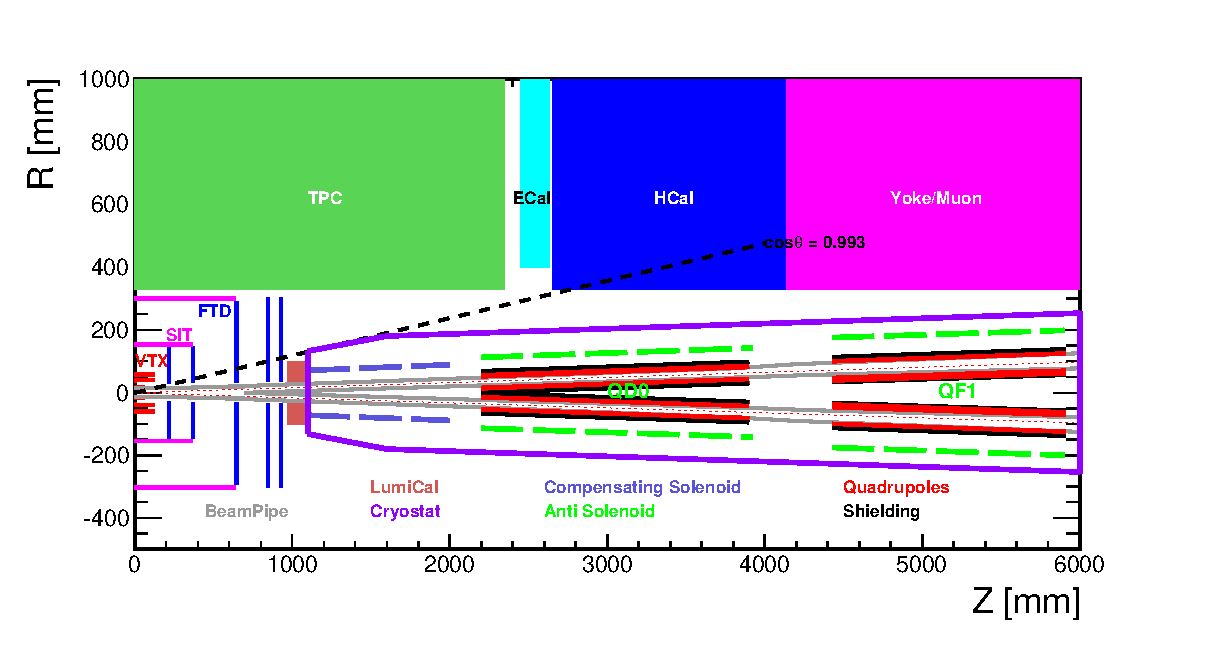
\includegraphics[scale=0.80] {Figures/MDI/mdi_IR_layout.eps}
	\caption{Layout of the interaction region.}
	\label{fig:mdi_IR_layout}
\end{figure}


\section{Final focusing magnets}
The two final focusing quadrupoles, QD0 and QF1, are inside the CEPC detector given the short focal length, and must operate in the background field of the detector solenoid. QD0 is the quadrupole magnet closest to the interaction point, with a distance of 2.2~m and 1.73~m in length. It is designed as double-aperture superconducting magnet realized with two layers of cos-theta quadrupole coil using Rutherford cable without iron yoke. The total four coils are clamped with stainless steel collars. It shall deliver a gradient field of 151~T/m and control the filed harmonics in the sensitive area to be below $3\times 10^{-4}$. The cross-sectional view of the single aperture of the QD0 is depicted in Fig.~\ref{fig:mdi_QD0_Structure}.

\begin{figure}[h!]
	\centering
	\includegraphics[scale=0.60] {Figures/MDI/mdi_QD0_Structure.png}
	\caption{Schematic view of the single aperture of the QD0 superconducting magnet.}
	\label{fig:mdi_QD0_Structure}
\end{figure}


\section{Detector backgrounds}
Backgrounds will impose significant constraints on the detector design and technologies to be adopted. Different backgrounds can give rise to primary particles that can enter the detector directly, or generate secondary particles that ultimately reach the detector. They can cause radiation damages to detector and electronics components, and degrade their particle detection performance. Moreover, backgrounds of high rate can increase the detector occupancy, and thus exaggerate the data-taking capability of the impaired detector. It is desirable to characterize backgrounds originating from different sources, and mitigate their impacts with effective and sufficient detector protection. Thorough studies with Monte Carlo simulation, together with lessons and experience learned from previous experiments, shall provide necessary guidance for detector and machine design optimization. Main backgrounds from beam-beam interactions, synchrotron radiation and beam-gas interactions are described.

\subsection{Beam-beam interactions}

\subsection{Synchrotron radiation}

\subsection{Beam-gas interactions}

\section{Luminosity instrumentation}
\label{sec:LumiCal}

Very forward region at CEPC will be instrumented with a luminometer (LumiCal) designed to enable integral luminosity measurement with a precision of $10^{-3}$ and $10^{-4}$ in $\epem$ collisions at 240~GeV center-of-mass energy and at the $\Zboson$-pole, respectively. The precision requirements on the integral luminosity measurement are motivated by the CEPC physics program, intended to test the validity scale of the Standard Model through precision measurements in the Higgs and EW sectors. Many sensitive observables for such measurements, critically depend on the uncertainty of the integral luminosity. Several technological options for LumiCal design are under study, as described in Sec.\textbackslash\{\} \textbackslash\{\}ref\{sec:lumi\_tech\}, with emphases on the precision of polar angle and energy reconstruction of Bhabha particles scattered in the $t$-channel \$V (V=\textbackslash\{\}gamma, \textbackslash\{\}Zboson)\$ exchange. Luminometer at CEPC is a precision device with challenging requirements on the mechanics and position control. Precision requirements on integral luminosity measurement set the precision of the opening aperture and positioning control of the LumiCal. Various sources of luminosity uncertainty in this respect are reviewed in Sec.\textbackslash\{\} \textbackslash\{\}ref\{sec:lumi\_systematics\}. Encouraging estimations on feasibility of the luminosity precision goals are presented. Detailed studies are ongoing, to include the full simulation of physics and machine induced processes and of the detector itself, for various luminometer positioning and technology choices.


\subsection{Systematic effects in the luminosity measurement}
\label{sec:lumi_systematics}
The main measure of luminosity at CepC is the count of Bhabha events $N_{Bh}$ detected in coincidence in the two halves of the luminosity calorimeter LumiCal. The luminosity figure is then obtained from the equation,
\begin{equation}\label{eq:lumi}
\mathcal{L} = \frac{N_{Bh}}{\sigma_{Bh}}
\end{equation}
where $\sigma_{Bh}$ is the cross section for the Bhabha process integrated over the same momentum acceptance region as used for the counting of Bhabha events. The limited precision with which the acceptance region is defined gives rise to a number of systematic effects. Further, other processes misidentified as Bhabha and the limited accuracy of the theoretical calculation of $\sigma_{Bh}$ contribute to the overall systematic uncertainty.

Theoretical accuracy of $\sigma_{Bh}$ is a matter of dedicated effort which can meaningfully be undertaken once a collider project is approved. In the past, the record accuracy of $5.4\times10^{-4}$ has been achieved for the OPAL experiment at LEP \cite{opal2000}, for the $\epem$ center-of mass (CM) energy of 91~GeV. This precision is sufficient for the Higgs program at CEPC, while higher precision may be required for the $Z$-pole run.

Beam interactions with the residual gas produce a background electrons and photons which are occasionally misidentified as Bhabha events. At LEP, this source of background was reduced by the selection criteria for the energy of detected particles. The quality of beam tube vacuum near the interaction region is crucial for this kind of background.

Two-photon exchange processes in which the products of the photon interaction escape down the beam pipe and the spectator electrons are misidentified as Bhabha electrons represent an important source of irreducible background to Bhabha counting. The contribution of such processes to $N_{Bh}$ is of the order of a few permille \cite{Boz13}. This must be corrected using models benchmarked against experimental results for the part of the final-particle phase space in which the products of the photon interaction are detected.

Precision of the definition of the acceptance region for the final Bhabha particles is affected by a number of effects, such as the size and the position of the interaction region, the accuracy of the manufacturing and the positioning of the LumiCal, beam energy spread and bias, mechanical vibrations, thermal stress which may affect the relative position of the LumiCal and the final beam focusing quadrupoles, and detector effects such as the precision and bias of the energy and position reconstruction.

A generator-level study was performed to assess the effects related to the precision of the Bhabha acceptance region on Bhabha counting. An underlying assumption of the study is the LumiCal concept in which the LumiCal has a cylindrical or conical geometry centered on the outgoing beam axis, the distance from the LumiCal front plane to the IP is 0.95~m, and the detector extends radially from 25 to 100~mm. It is further assumed that for final Bhabha particles hitting the radial region between 50 and 75~mm (the fiducial volume, FV) shower leakage has a negligible effect on the reconstruction of the polar angle and the energy.

For the study, Bhabha event samples were generated using the BHLUMI generator \cite{Bhlumi97}. CM energy of 240~GeV was assumed, corresponding to the CM energy of the Higgs program at CepC. The particles were generated in the range of polar angles including a $\sim7\;\mathrm{mrad}$ margin outside the FV to allow non-collinear FSR to contribute to the events. After event generation, smearing is applied to the final particle vertices and momenta according to the nominal CepC parameters \cite{cepcweb}. Additional smearing or bias is then applied according to one systematic effect at a time. Four momenta of close-by particles are summed up to account for cluster merging in LumiCal.

The average Bhabha count in the mirrored asymmetric polar-angle acceptance regions, such as applied at OPAL \cite{opal2000}, is taken as $N_{\mathrm{Bh}}$. A minimal energy of $1/2E_0$ is required of the final particles, where $E_0$ is the nominal beam energy. The assumption that the LumiCal halves are centered on the outgoing beam axis is crucial for the application of the OPAL counting method, as well as for a reliable data-driven control of the radial offset of the LumiCal.

Fig.~\ref{fig:bes} shows the Bhabha counting bias as a function of the width of the longitudinal boost distribution due to the beam energy spread. Results for full fiducial acceptance and for the OPAL-style counting algorithm are shown. If Bhabha events are accepted in the full fiducial volume, counting correction is required for which the beam energy spread must be known to within 10\%. On the other hand, the OPAL counting algorithm is practically invariant to the beam energy spread. In general, the OPAL counting leads to an effective cancellation of left-right asymmetries of the acceptance region.

\begin{figure}
	\centering
	\includegraphics[width=0.9\textwidth]{Figures/MDI/beamEnergySpread}
	\caption{Bhabha counting bias as a function of the width of longitudinal boost distribution due to the beam energy spread. }
	\label{fig:bes}
\end{figure}

It has been shown that most requirements on the LumiCal manufacturing and positioning, as well as on the MDI and beam delivery needed to reach the luminosity precision of 1 permille are technically feasible with the present state of the art of accelerator and detector technology. The most important challenge identified is the precision of the inner acceptance radius $r_{\text{in}}$ of LumiCal. In order to keep the luminosity precision of 1 permille, $r_{\text{in}}$ must be known to within $10\,\mathrm{\mu m}$. The precision requirement of $r_{\text{in}}$ scales linearly with the required luminosity precision, implying a correspondingly stricter requirement for the $\Zboson$-pole run.


% -------------------------------------------------------Sec 2   ----------
\subsection{Luminosity detector options }  %----------------

A Bhabha event is measured for a pair of low angle $e^+$ and $e^-$ of beam energy, back-to-back to the interaction point. Therefore, the luminosity detector is instrumented with a pair of forward calorimeters, as is illustrated in Fig.~\ref{fig:opal_siw}, in fine segmentation for measurement of the electron impact position in $r-\phi$ plane. The OPAL Si-W calorimeter is also shown in Fig.~\ref{fig:opal_siw} to demonstrate the most compact assembly that can be made of sandwiched silicon wafers and tungsten layers.The silicon wafer is segmented in wide strips of 2.5 mm in radius and 11.25$^\circ$ in polar angle \cite{OPAL_SiW}.

\begin{figure*}[b!]
	% \vspace{.5cm}
	\centering
	\includegraphics[width=.45\linewidth]{Figures/MDI/Bhabha_lumical.png} 
	\hspace{.5cm}
	\includegraphics[width=.35\linewidth]{Figures/MDI/opal_siw.jpg} 
	\vspace{.2cm}
	\caption{   The detection of Bhabha events by forward LumiCal detectors is illustrated on the right. The OPAL Luminosity calorimeter is shown on the right for a active silicon layer with silicon strip detectors segmented in 2.5 mm x 11.25$^\circ$ wide strips.  
		\label{fig:opal_siw} }
\end{figure*}


Silicon strips are used for detection of electron impact position. If the hit is between strips, the ionization charges along the electron traversing pass are drifting to the adjacent strips and is ambiguous in its impact position. Events within the strip gap become a major systematic error on event counting for a fiducial region drawn by the edge of a strip.

Illustrated in Fig.~\ref{fig:strip_gap} are results of a test-beam investigation on charge-sharing between strips of prototype detectors originally made for the CMS preshower detector (shown in Fig.~\ref{fig:strip_gap}).The silicon wafers are 65x65 mm$^2$ implemented with 2 mm wide strips. The gaps between strips are implemented for charge collection tests, with the widths of 50 or 160 $\mu$m.

In the beam tests, a set of tracking telescope provides reference position by extrapolation on a test sample. A charged particle traversing a silicon wafer (380 $\mu$m, in this case) generates about 25k electron-hole paired drifting toward the p-n electrodes by the reverse-bias voltage applied. The charge collection are compatible and are 100 \% through the regions of strip implantation and between strips where the ionization charge are drifted to the adjacent strips (middle). The ionization charge are distributed in a very narrow cone of about 20 $\mu$m in diameter; as a result, the charges tend to flow totally to the nearest strip. This is seen by the charge sharing parameter, $\eta = Q_r/(Q_r+Q_l)$, to the two adjacent strips that peaks near 0 or 1 (Fig.~\ref{fig:strip_gap}.right).

The test beam particles are randomly distributed across the gap between strips. The $\eta$ distribution illustrates that one can hardly determined the particle hit position between the gap. It is also interesting to see the compatible distributions for the gaps of 160 $\mu$m or 50 $\mu$m, meaning that the field degradations from the strip edge to the middle of the gap are compatible despite the widths.


\begin{figure*}[b!] 
	% \vspace{.5cm}
	\centering
	\includegraphics[width=.22\linewidth]{Figures/MDI/CMS_preshower.jpg} 
	\hspace{.2cm}
	\includegraphics[width=.28\linewidth]{Figures/MDI/CMS_strip_Q.png}  
	\hspace{.2cm}
	\includegraphics[width=.40\linewidth]{Figures/MDI/CMS_strip_gap.png} 
	\vspace{.2cm}
	\caption{  
		Beam tests using prototype silicon wafer of the CMS preshower detector (right) were conducted for collection of ionization charges generated by traversing particles across the gap between strips. The charge sharing by adjacent strips are plotted (middle) to the reference impact position (extrapolation of a upstream telescope). The sum strip charges (middle plots) is compatible to the hits on a strip. The charge sharing in $\eta Q_r/(Q_r+Q_l)$ peaks near 0 and 1,
		indicating non-linear response to the randomly distributed beam particles across the gap \cite{CMS_2000-042}.
		\label{fig:strip_gap} }
\end{figure*}

The counting of Bhabha events cares about particle hits with in fiducial cuts, and not the spatial resolution of each events. In the case of test beam with the incident particle distributed randomly (flat) across the gap, the $\eta$ distribution is symmetric and the integrated in half (divided by $\eta=0.5$) is about equal. The middle point of the gap is corresponds to $\eta=0.5$ that can be chosen as the fiducial cut between two strips. The situation at CEPC would be complicated by the magnetic field to tilt the $\eta$ distribution into non-symmetric, and therefore the difficulty to decide on the fiducial cut in a gap between two strips.

The choice of using fine-pitch silicon strip detectors would have improve the spatial resolution for detecting Bhabha electrons. Silicon strip detectors are implemented, e.g. in 25 $\mu$ pitch with gap of $\sim 10$ $\mu$m, and the readout bonding of every other strips (50 $\mu$m pitch) as is shown in Fig.~\ref{fig:strip_detector}. Strip detector of this type reaches $\sim 5$ $\mu$m intrinsic resolution for incident position of a charge particle. The $\eta$ distribution is peaking at edge as the case of wide-strip detector (Fig.~\ref{fig:strip_detector}). By characterizing the sharing in $\eta$, the error on fiducial cut in position is error on mean of the intrinsic resolution and is much better than 5 $\mu$m.

\begin{figure*}[t!]  % slides 0915
	% \vspace{.5cm}
	\centering
	\includegraphics[width=.28\linewidth]{Figures/MDI/strip_cutview.png} 
	\hspace{.4cm}
	\includegraphics[width=.25\linewidth]{Figures/MDI/strip_implant.png}  
	\hspace{.4cm}
	\includegraphics[width=.34\linewidth]{Figures/MDI/strip_eta.png} 
	\vspace{.2cm}
	\caption{  
		Silicon strip detector: (left) ionization charge collection by strips in revise bias of P-N junction; (middle) the strip implantation and readout of every other strips; charge share of a hit between strips expressed by $\eta=Q_r/(Q_r+Q_l)$. The ionization charge can be collected by a several strips. The $\eta$ distribution is also plotted for two-strip (dotted) and three-strip (dashed) cases. The floating strip between two readout strips creates a coupling in field to drive ionization charges toward both strips. Without it, the $\eta$ peaks toward the edges expelling distribution in the $\eta\sim 0.5$ region.
		\cite{NIM_reso}.
		\label{fig:strip_detector} }
\end{figure*}


%----------------------------------------------------  


%------------------------------------------------------------------ 
\subsection{Tracking of Bhabha electrons to 10$^{-4}$ precision}   %-----------------------------------------
\label{sec:BhabhaTrcking} % 0915 slides

The alignment of LumiCal along the beam line in z is expected
to be better than 100 $\mu$m, correspond to an offset in $\theta$ of 
$\theta=30$ mRad at $z=1$ m, which is equivalent to 3 $\mu$m in radius.
The dominant systematic uncertainties for detection of Bhabha events are  
\begin{list}{}{\setlength{\leftmargin}{18pt}
		\setlength{\labelsep}{10pt}
		\setlength{\itemsep}{5pt}
		\setlength{\parsep}{0pt}}
	\item{i)}
	detector alignment errors in r, $\phi$ and in z;
	\item{ii)}
	multiple scattering in upstream materials;
	\item{iii)} 
	spatial resolution of electron impact position ($\theta$ angle).
\end{list}
Each of the error can not be realized by a stand-alone LumiCal
without an external calibration system. 
In the following, we suggest adding a low-angle diamond or silicon ring
before the LumiCal to build a simple 3-point tracking system for electrons,
so as to calibrate the geometrical off-sets of the LumiCal.
Illustrated in Fig.~\ref{fig:Bhabha_tracking} is a sketch showing
the three points of electron positions.
The IP is where electron track initiates.
The diamond ring can be independently mounted in front of the LumiCal.
Assuming that the diamond is made of two rings in radius, and
thus provides an edge for calibration.
The tracking of two-point extrapolation to the LumiCal shows the off-sets 
to be adjusted, and also the distribution fiducial cut in $\theta$
to be sorted for the mean of error.

The IP position can be measured and calibrated by events of multiple jets.
The distribution is illustrated in Fig.~\ref{fig:Bhabha_tracking} assuming
a Gaussian distribution. Assuming the diamond is segmented in radius.
Events on the edge can be separated, extrapolated on the LumiCal, to be
identified and compared for the predicted position on LumiCal.

The precision on luminosity matters mostly by the precision on 
the lower bound of $\theta_{min}$ cut for event selection in fiducial region.
Therefore the spatial resolution of the electron impact position on LumiCal
shall be pursued. One may apply the mature technology of silicon strips
in readout pitch of 50 $\mu$m to reach a detector intrinsic resolution of
5 $\mu$m. It is illustrated in Fig.~\ref{fig:Bhabha_tracking} for front layers
of the LumiCal from the inner radius, in a span of about 20 mm. 
The mean on the error of $\theta_{min}$ would be much smaller.




\begin{figure*}[t!] 
	\vspace{.5cm}
	\centering
	\includegraphics[width=.66\linewidth]{Figures/MDI/Bhabha_tracking.png}  
	\hspace{.2cm}
	\includegraphics[width=.24\linewidth]{Figures/MDI/Bhabha_Si_fine_pitch.png} 
	\vspace{.2cm}
	\caption{  Tracking of Bhabha electrons is suggested for the precision
		to $10^{-4}$ on the mean of error for the fiducial $\theta$ cut,
		which corresponds to $\sim 1$ $\mu$m in radius for the LumiCal
		at Z = 1 m.
		Diamond or silicon are implemented between the $e^+ e^-$
		interaction point and the LumiCal with Silicon strip
		of 5 $\mu$m precision. 
		The alignment of LumiCal is calibrated by the 
		tracking of three points: IP, diamond/si ring, and LumiCal front face
		for the mean of error on $\theta$ to better than 1 $\mu$m,
		to reach $10^{-4}$ in precision for luminosity measurement.
		\label{fig:Bhabha_tracking} }
\end{figure*}


\begin{figure}[p!] 
%	\vspace{.5cm}
%	\centering
%	\includegraphics[width=.42\linewidth]{Figures/MDI/CEPC_ring.png}  
%	\hspace{.2cm}
%	\includegraphics[width=.44\linewidth]{Figures/MDI/beampipe0926.png} 
%	\vspace{.2cm}
%	\caption{  The CEPC has a double ring at interaction point
%		with a beam cross angle of 33 mRad. The accelerator configuration
%		and the beam pipe sketch at interaction point are shown.
%		\label{fig:beamcrossing} }
%	% \end{figure*}
	
	% \begin{figure*}[b!]    % 0901 slides
%	\vspace{.5cm} 
	\centering
	\includegraphics[width=.35\linewidth]{Figures/MDI/BH_rphi.png}  
	\hspace{.2cm}
	\includegraphics[width=.35\linewidth]{Figures/MDI/BH_b2b.png} 
	% \vspace{.2cm}
	\caption{ Bhabha events of
		BHlumi simulation at Z-pole are plotted for the 
		center of mass (red) and the beam-crossing boosted (blue)
		distribution on a LumiCal surface (left) and the back-to-back angle.
		\label{fig:Bhabha_33mrad_offset} }
	% \end{figure*}
	
	% \begin{figure*}[h!] 
	\vspace{.5cm}
	\centering
	\includegraphics[width=.35\linewidth]{Figures/MDI/BH_b2b_phi.png}  
	\hspace{.2cm}
	\includegraphics[width=.35\linewidth]{Figures/MDI/BH_b2b_the.png} 
	% \vspace{.2cm}
	\caption{ Bhabha events are 
		selected in $\phi$ angles after boost by the beam crossing angle
		for both electrons (red) and positrons (blue) on each side
		of the LumiCal $r-\phi$ plan at $z=1$ m, and the corresponding
		$\theta$ angle distributions.
		\label{fig:Bhabha_33mrad_offset2} }
\end{figure}


%------------------------------------------------------------------ 
\subsection{Boost by beam-crossing to Bhabha electrons }   %-----------------------------------------
\label{sec:beamcross_boost} %  

The double ring configuration  of the CEPC 
machine design at interaction point has a beam crossing angle of 33 mRad.
%%as is illustrated in Fig.~\ref{fig:beamcrossing}.
The effect to elastic scattering Bhabha events is a boost of center-of-mass (CMS)
off the ring center, corresponding to an off-set by 16.5 mRad in horizontal
direction to both the electrons and positrons.
The boost effect to scattered electrons on the LumiCal front face at $z=1$ m
is illustrated in Fig.~\ref{fig:Bhabha_33mrad_offset}. The angular distribution
of Bhabha events is simulated with the BHlumi~\cite{BHlumi} program.
The back-to-back distribution after the boost is also plotted, which peaks
at 33 mRad off the CMS distribution.

A Bhabha event is detected requiring both electron and positron detected.
The boost pushes low angle (on -x direction) electron (positron) into the beam pipe,
and is lost from detection. Therefore, the corresponding angle to be detectable is
widen. Illustrated in Fig.~\ref{fig:Bhabha_33mrad_offset2} are the distributions of
boosted electrons (red) and positrons (blue) selected with the electrons
on horizontal ($\phi=0$) to diagonal ($\phi=135^\circ$) directions.
For example, on the horizontal axis, the positron at CMS shall be generated with 
$\theta>36.5$ mRad to be detectable after being boosted to 20 mRad in laboratory,
and correspondingly, the electron is booted to 53 mRad.
The correlation of $\theta$ angles of electrons and positron in laboratory frame
are also plotted in Fig.~\ref{fig:Bhabha_33mrad_offset2}.

In order to have sufficient Bhabha events (>50 nb) for luminosity measurements,
the $\theta_{min}$ of fiducial at CMS shall be $<35 $ mRad, in the case of circular
beampipe and detector inner radius. The design of the CEPC beampipe is in X-shape 
for beam crossing (Fig.\ref{fig:beamcrossing}).
The LumiCal is likely having a oval shape inner radius at $z=1$ m, with the horizontal 
radius of 50 mm. 
It should be pursued for the smallest radius possible,
so as to gain the Bhabha detection cross section.



%------------------------------------------------------------------ 
\subsection{Shower leakage of LumiCal to tracking volume}   %-----------------------------------------
\label{sec:showerleak} %   slides 0811

%%The LumiCal in the Machine-Detector Interface region
%%is illustrate in Fig.~\ref{fig:CEPC_cutview}.
The LumiCal is mounted in front of the Quadruple magnet with
the front plane at $z= \pm 1$ m.
The central detector tracking volume is, however, 
surrounding the beam pipe extended to $z= \pm 2$ m. 
The electron shower at the edge of outer radius will cause
shower leakage into the tracking volume.


%\begin{figure*}[b!] 
%	\vspace{.5cm}
%	\centering
%	\includegraphics[width=.40\linewidth]{Figures/MDI/beam_z.png} 
%	\hspace{.5cm}
%	\includegraphics[width=.52\linewidth]{Figures/MDI/lumical_z.png} 
%	% \vspace{.2cm}
%	\caption{The LumiCal mounted in front of the quadrupole magnet 
%		is located with the back plane at $z= 1.11$ cm from the interaction point.
%		\label{fig:CEPC_cutview} }
%\end{figure*}

The shower leakage off the LumiCal is investigated with a GEANT 
simulation assuming a Si-W sandwiched LumiCal stacked with twenty 
decks of 2mm air-gap and $1 X_0$ tungsten (3.5 mm thick). 
The air-gap is inserted with a layer of silicon wafers of 0.3 mm thick.
The front layer of the LumiCal is positioned at $z=1$ m.
The GEANT code was developed with good agreement for a beam test study of
lateral shower distributions of 2 to 50 GeV electrons measured by a fine pitch 
silicon strip detector \cite{NIM_lateral}. 
The GEANT simulation parameters in used are listed in
Table~\ref{tab:g3_parameters}. 

%----------------------------------------------------slides  0811
\begin{table}[t!]
	% \vspace{0.5cm}
	\centering
	\begin{tabular}{   ccccc | ccc }
		\hline
		\hline 
		LOSS & MULS & BREM & PAIR & DRAY &  GUTGAM   & CUTELE   & DCUTE \\
		\hline
		1 & 2 & 1 & 1 & 1 &  0.01 MeV & 0.01 MeV & 0.2 MeV \\
		\hline
		\hline
	\end{tabular}
	\caption{ Parameters of the GEANT simulation applied for the LumiCal
		shower leakage study.
		\label{tab:g3_parameters} }
\end{table}


\begin{figure*}[th!] 
	\vspace{.5cm}
	\centering
	\includegraphics[width=.50\linewidth]{Figures/MDI/g3_event_display.png}   
	\vspace{.2cm}
	% \vspace{.2cm}
	\caption{ A GEANT simulation event of a 50 GeV electron shower on
		a LumiCal stacked with 20 decks of silicon and Tungsten layers.
		It is coded using a beam test study for electron shower. 
		The outer cone corresponding to the $\cos\theta=0.992$ angle 
		separating MDI to TPC volume.
		\label{fig:g3_event} }
\end{figure*}


Illustrated in Fig.~\ref{fig:g3_event} is an event display of the simulation.
The cone surrounding the LumiCal corresponding to $\cos\theta=0.992$ 
($\theta=126.6$ mRad) separating MDI to the central tracking volume.
The cone is implemented as is made of 5 mm Fe with active scintillator 
layer on both surfaces for detection of shower secondaries passing through. 
The geometry of the LumiCal is configured in a TUBE with uniform radius,
and a CONE shape with outer edge at a constant angle to IP.
The CONE shape is intended for minimizing the shower leakage.
The parameters of the two configurations are:
\begin{list}{}{\setlength{\leftmargin}{18pt}
		\setlength{\labelsep}{10pt}
		\setlength{\itemsep}{5pt}
		\setlength{\parsep}{0pt}}
	\item{i)}
	a TUBE shape with tungstan layer or radius $r=25-100$ mm;
	\item{ii)}
	a CONE shape with the outer radius extended radially from $z=0$
	to angle span to 100~mm at $z=1$~m ($atan.(10./100.)$.
\end{list}



\begin{figure*}[bh!] 
	% \vspace{.5cm}
	\centering
	\includegraphics[width=.30\linewidth]{Figures/MDI/TUBE_lateral.png}   
	\hspace{.5cm}
	\includegraphics[width=.45\linewidth]{Figures/MDI/TUBE_lateral_p.png} 
	\vspace{-.2cm}
	% \vspace{.2cm}
	\caption{ Simulation of 50 GeV electrons at fixed incident angles 
		on a TUBE shape LumiCal is plotted for 
		(left) lateral show profiles on the first 10 decks of silicon wafer,
		(right) and the momentum distributions of shower secondaries passing
		the 5 mm Fe cone at $\cos\theta=.992$, the the hit positions in $r$, $z$.
		\label{fig:TUBE_leak} }
	% \end{figure*}
	
	% \begin{figure*}[th!] 
	\vspace{.5cm}
	\centering
	\includegraphics[width=.30\linewidth]{Figures/MDI/CONE_lateral.png}   
	\hspace{.5cm}
	\includegraphics[width=.45\linewidth]{Figures/MDI/CONE_lateral_p.png} 
	\vspace{-.2cm}
	% \vspace{.2cm}
	\caption{ Simulation of 50 GeV electrons at fixed incident angles 
		on a CONE shape LumiCal is plotted for 
		(left) lateral show profiles on the first 10 decks of silicon wafer,
		(right) and the momentum distributions of shower secondaries passing
		the 5 mm Fe cone at $\cos\theta=.992$, the the hit positions in $r$, $z$.
		\label{fig:CONE_leak} }
\end{figure*}

The simulation has assumed the front plane of LumiCal extended to 100 mRad
from the IP. A electron shooting the edge of outer radius the TUBE configuration
is not contained, with energetic shower secondaries escaping into the gap to the
tracking volume. The CONE configuration provide better coverage with 
the shower center contained in the full thickness of the calorimeter. 
In Fig.~\ref{fig:TUBE_leak} the lateral shower profiles are shown
for 50 GeV electrons at edge of the TUBE LumiCal. 
The shower center of a electron shooting at 95 mRad escapes the calorimeter
after about half the depth (10 decks). 
When the shower is full contained (shooting at 40 mRad), the shower leakage
is minimal (right plots) and the momenta of shower secondaries reaching the 
iron cone at $\cos\theta=.992$ are below 30 MeV. 
The shower leakage of a 95 mRad electron at 95 mRad spreads over the icon cone
to $z=2$ m, and the momentum distribution reach up to 100 MeV.
The 5mm Fe of the cone absorbs shower secondaries by a factor of three.
The distributions before and after the Fe cone at $\theta=.992$ are compared 
in  Fig.~\ref{fig:TUBE_leak}.

The CONE shape design of LumiCal in intended to maximize the shower containment
with the edge of outer radius fixed to 100 mRad radially from the IP, so that the 
shower center in fragmentation stays within the calorimeter volume.  
A denser calorimeter 
(e.g. by reducing the width of air-gap in the Si-W stacking) shall have
the shower secondaries distributed narrower. 
In Fig.~\ref{fig:CONE_leak} the distributions are made with electrons 
generated in the same condition as for the TUBE LumiCal simulation.
The difference in distributions of shower secondaries is narrower in $z$,
for electrons at the edge (95 mRad).
However, with the electron shooting further outward (99 mRad) on the edge, 
the shower leakage observed by the Fe-cone increases at
$\sim z=1.1$ m.

A TUBE LumiCal has uniform dimension of parts that is convenient for construction.
The shower leakage is maximum when the shower center leaks off the middle layers
of LumiCal, in which the energetic secondaries are along the electron
incident direction scattered downstream, and may have escaped going into 
TPC tracking volume.
Comparison of the shower leakage into the Fe-cone and traversed through 
are listed in Fig.~\ref{fig:leak_fraction} for 50 and 125 electrons versus the
incident angles to the LumiCal. 
When the shower is well contained, the leakage is just a few dozens of 
less than 30 MeV particles.  A shower on the edge creates up to 3k 
shower secondaries into the tracking volume mostly of less than 100 MeV.
The 5 mm Fe cone can filter a large fraction of them, to less than 1k particles
traversing through.





\begin{figure*}[th!] 
	% \vspace{.5cm}
	\centering
	\includegraphics[width=.40\linewidth]{Figures/MDI/shower_leak_50.png}   
	\hspace{.5cm}
	\includegraphics[width=.405\linewidth]{Figures/MDI/shower_leak_125.png}   
	\vspace{-.2cm}
	% \vspace{.2cm}
	\caption{ Average numbers of shower secondaries which leak into a 5 mm Fe-cone
		at $\cos\theta=.992$ versus at incident angles of 50 and 125 GeV electrons.
		The numbers are counted for particles traversing before and pass the 5 mm Fe-cone.
		\label{fig:leak_fraction} }
\end{figure*}





\section{Detector integration}






\bibliographystyle{Style/atlasnote} %% plain.bst
\bibliography{Chapters/MDI} %% bsample.bib

